\documentclass{article}
  \usepackage{ctex, graphicx, float}
\begin{document}
  \section{CompoNet结构说明}
  \subsection{功能}
    接受一段音符序列,对其进行“续写”。
  \subsection{输入}
    我们在已有的mid文件中随机选取了一些统计了音符的四个
    要素(pitch,dynamic,rhythmValue,duration)的分布情况如下图所示:
    
    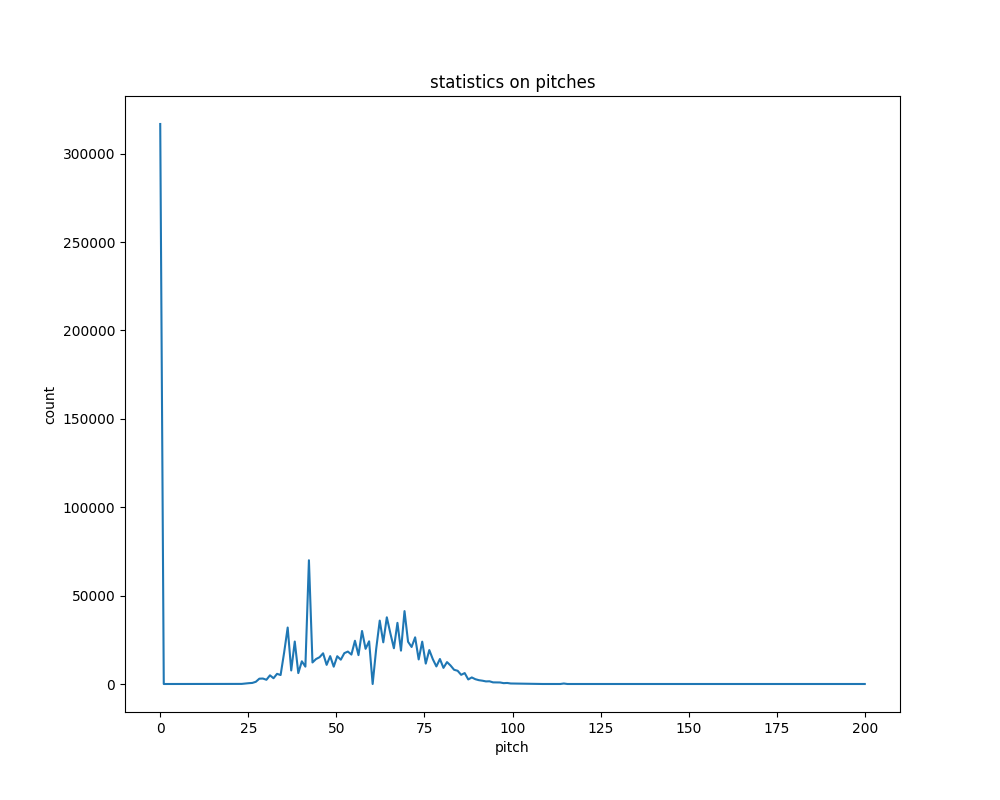
\includegraphics[width=.9\textwidth]{picture/pitches.png}
      
    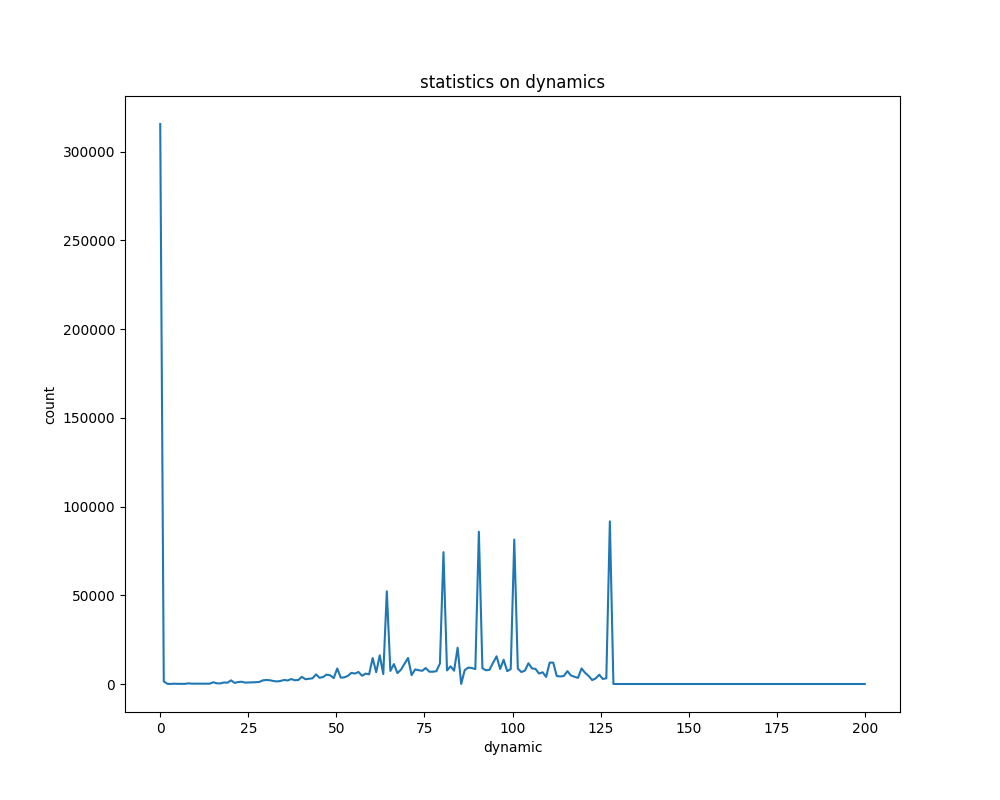
\includegraphics[width=.9\textwidth]{picture/dynamics.png}

    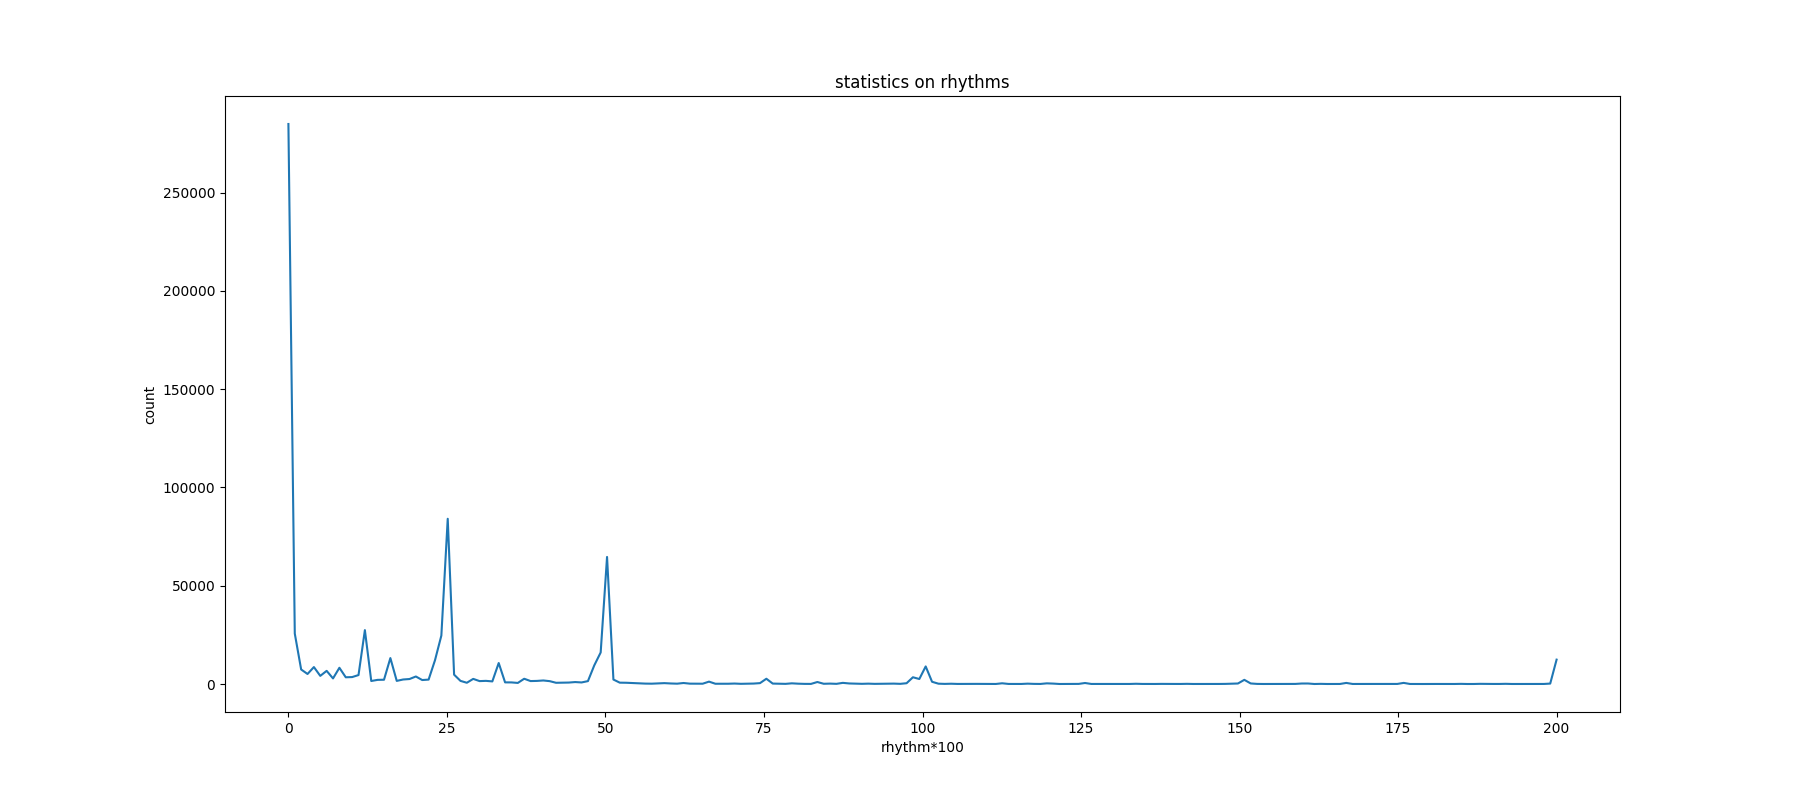
\includegraphics[width=.9\textwidth]{picture/rhythms.png}
    
    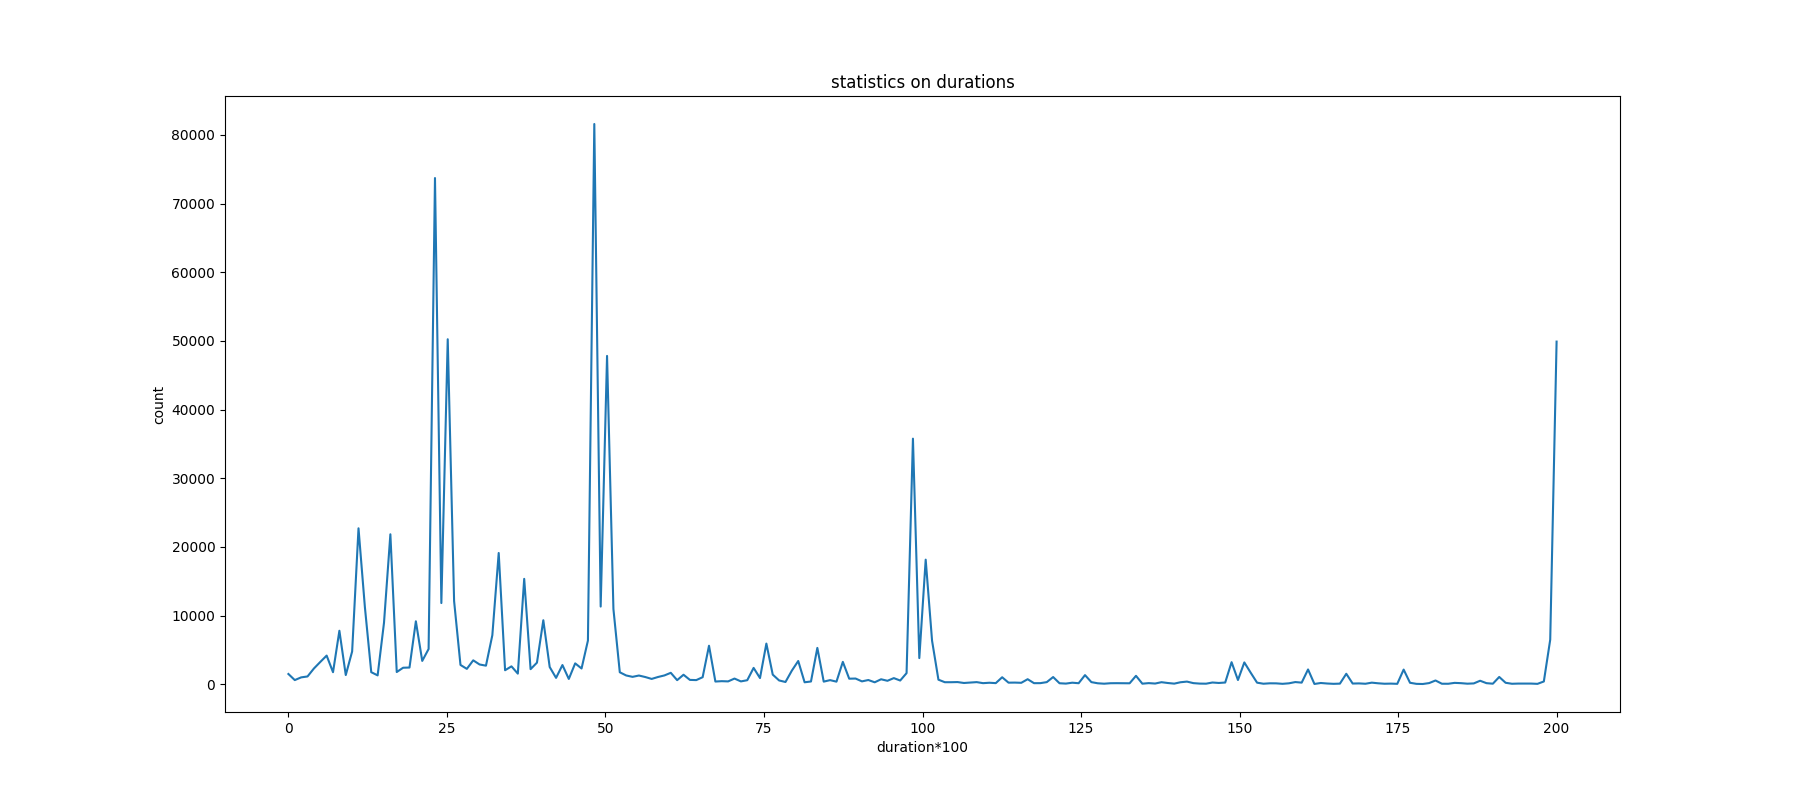
\includegraphics[width=.9\textwidth]{picture/durations.png}

    可以看出,虽然rhythmValue和duration的取值理论上是连续的,但实际上取到的值很有限,
    因此可以认为这四个要素都是离散的。基于这个事实,
    为了能够进行随机取样和关于“信息密度”的直觉判断,
    我们对输入的四个要素先分别进行one-hot编码,再连接成一个向量作为神经网络的输入。

  \subsection{结构和训练}
    我们模仿char-rnn-tensorflow构建了一个两层、每层128个神经元的递归神经网络,在输出处增加了一个隐层
    将其输出变换为和输入向量相同的长度,然后拆分为四个部分,对每部分计算softmax,
    得到音符的每个要素所有取值的概率分布,然后将其与下一个音符的one-hot编码计算交叉熵作为
    损失函数。
  \subsection{取样}
    在取样时,我们对四个要素分别进行取样。如前所述,神经网络给出了下一个音符四个要素的每种取值的概率,为了提高输出的质量,我们只考虑概率大小在平均值以上的可能取值。
  \subsection{效果}
\end{document}
